%%==============================================================================
%  Model exercise Desiccation under in-situ conditions
%  HS, 05/04/2019
%%==============================================================================
\section[MEX 1-3: Desiccation under in-situ conditions]{Model Exercise 1-3: Desiccation under in-situ conditions}
\label{sec:mex12}
\index{desiccation process}
%------------------------------------------------------------------------------
\Authors{Holger Steeb}
%------------------------------------------------------------------------------

We focus on in-situ (image-based) characterization of desiccation processes of sandy-clay samples under confined conditions. The samples under investigation have to be prepared in sizes small enough for high-resolution X-Ray Computed Tomography (XRCT) and large enough to be representative.

%\begin{wrapfigure}{l}{8cm}
\begin{figure}[ht!]
\centering
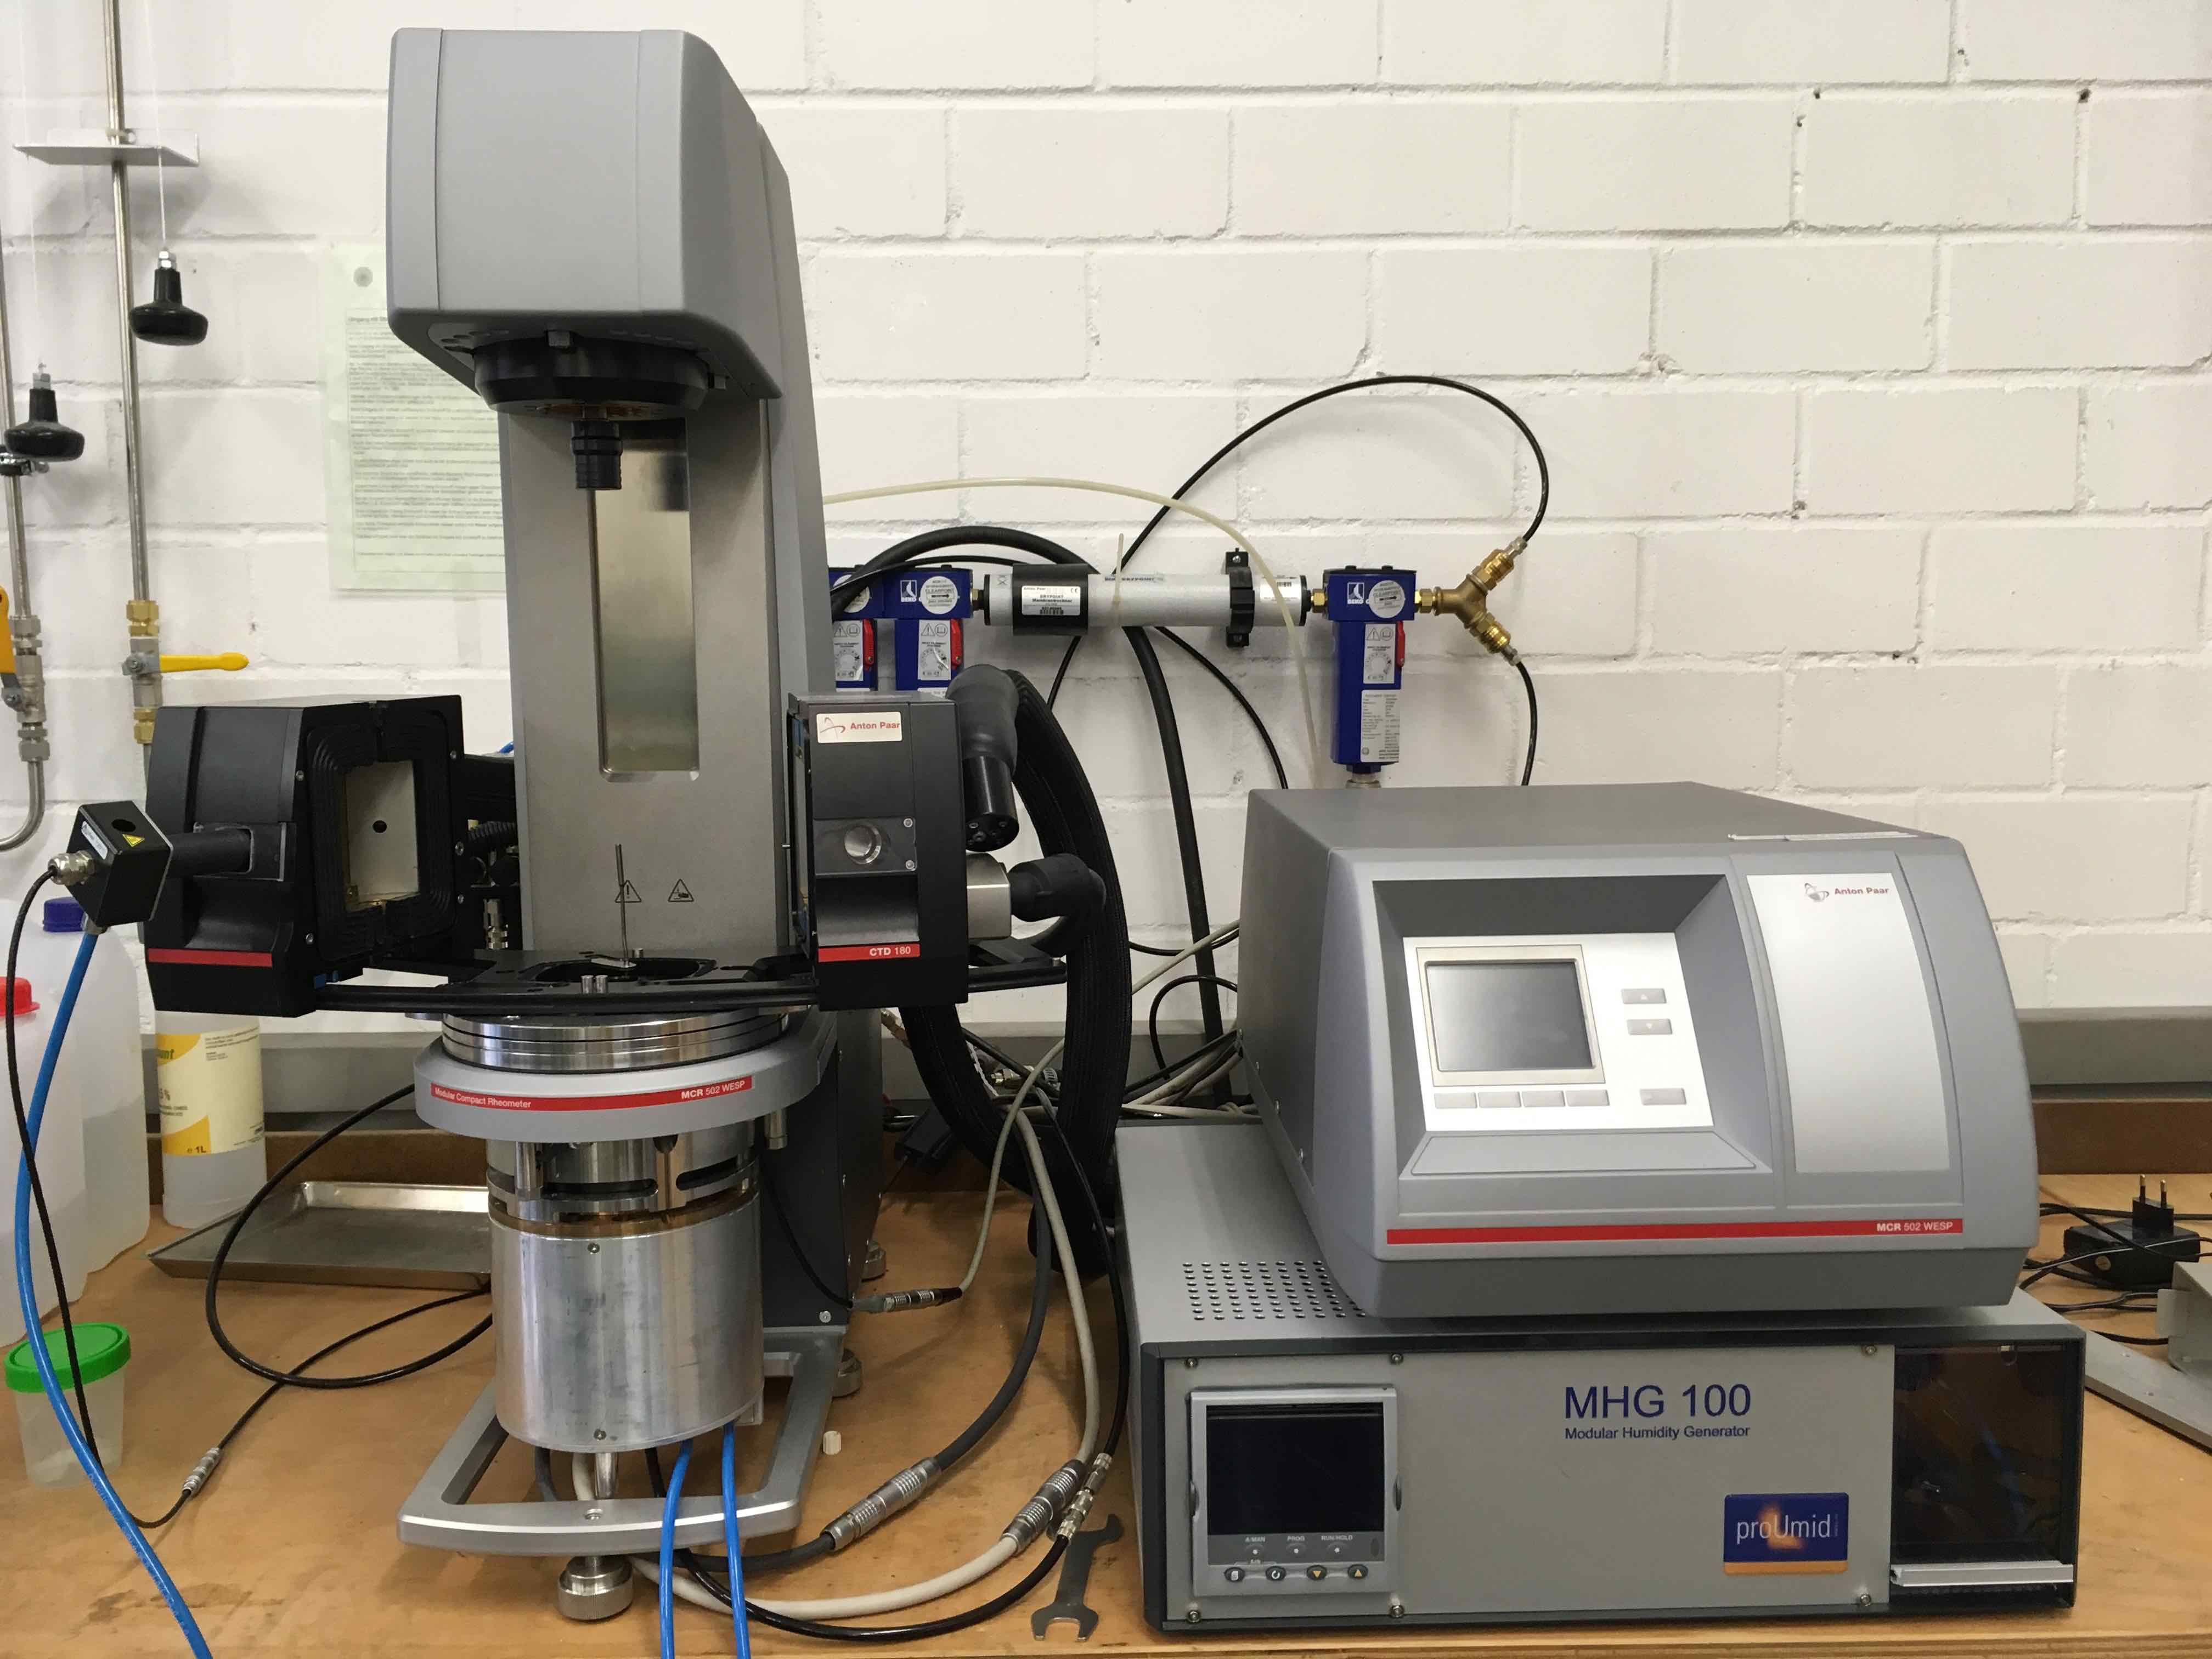
\includegraphics[width=8cm]{figures/mex_013_small.png}
\caption{Anton Paar MCR~502 TwinDrive DMTA-rheometer with ProUmid MHG~100 humidity controller.}
\label{fig:env_chamber}
\end{figure}
%\end{wrapfigure}

\begin{list}{-}{\leftmargin=1em \itemindent=0em \itemsep=0em}
\item A cylindrical clay core with diameter $D=30$ mm and height 
$H=60$ mm (or smaller to get a higher spatial resolution) is embedded in a hollow PEEK (Polyether ether ketone) tube. 
The sample is prepared with a drill hole of $d=5$ mm.
\item Further, the sample is firstly sealed with a Teflon shrink tube. Secondly the gap between the sample and the PEEK tube is filled with an epoxy resin.
Epoxy and PEEK have low X-Ray absorption properties. Through the embedding, radial deformations of the clay sample are preventing. 
\item The top and bottom parts of the samples are hydraulically sealed with end-caps corresponding to undrained conditions. The end-caps allow for axial deformations occurring during the shrinkage process. The drill hole is ``open''  allowing for water release/uptake.
\item The prepared sample with in-situ humidity (partially saturation) is placed in an environmental chamber (Anton Paar, CDT 100, Peltier heated), cf. Figure~\ref{fig:env_chamber}. Temperature and humidity is controlled (ProUmid MHG 100 humidity controller, ProUmid). 
\item If necessary, a small van has to be placed in the enironmental chamber allowing for controlled humidity convection in the drill hole. 
\item Drying/desiccation will be image-based characterized within the open XRCT scanner in Stuttgart. Therefore, the drill hole is temporary sealed.
\item We are aiming for a spatial resolution of $30 / 2500$ = 12 $\mu$m / voxel. XRCT scans will be performed for equilibrium states at certain humidity conditions (at ambient temperature of $\Theta = 20^o$ C).
\end{list}
